%%%%%%%%%%%%%%%%%%%%%%%%%%%%%%%%%%%%%%%%%%%%%%%%%%%%%%%%%%%%%%%%%%%%%%%%%%%%%%%%%%%%%%%%%%%%%%%%%%%%
% ==================================================================================================
% --------------------------------------------------------------------------------------------------
\chapter{Voxel-Wise Logistic Regression}\label{ch-vlr}
This section presents the proposed classification model
-- Voxel-wise Logistic Regression (VLR) --
in more detail, and explores the specific parameters and regularization strategies
requiring optimization.
\par
To review, the predicted lesion class label image $\hat{C}(x)$ is defined
using the subject-specific features $\bY(x) = {[1,Y^1(x),\dots,Y^\sk(x)]}^T$
and the corresponding model weights $\bb(x) = {[\b^0(x),\b^1(x),\dots,\b^\sk(x)]}^T$,
\begin{equation}
  \hat{C}(x) = \frac{1}{1+e^{-\eta(x)}},\qquad\eta = {\bb(x)}^T\bm{Y}(x).%
  \label{eq:eq:vlrmodel}
\end{equation}
While the implementation used for experimentation in this work
uses only one feature image ($K=1$), the FLAIR graylevel,
the derivations and discussions below will maintain generality for any selection of features.
%%%%%%%%%%%%%%%%%%%%%%%%%%%%%%%%%%%%%%%%%%%%%%%%%%%%%%%%%%%%%%%%%%%%%%%%%%%%%%%%%%%%%%%%%%%%%%%%%%%%
\section{Model Fitting}\label{ss:modelfitting}
Fitting the VLR model involves estimating $\bb$ for each voxel $x$.
This requires some training data:
feature vectors from a population of $N$ observations $\bY(x) = \{\bY_1(x),\dots,\bY_{\sn}(x)\}$,
and the corresponding labels $\C(x) = \{C_1(x),\dots,C_{\sn}(x)\}$. 
As in many probabilistic models,
parameter estimation involves maximizing the likelihood of the model, given this data --
i.e.\ maximum likelihood estimation (MLE).
% ==================================================================================================
\subsection{Challenges}\label{ss:vlr-chmle}
Three major challenges emerge during model fitting.
These challenges involve contradictions between prior knowledge
and the fitted model using the available training data.
That is, these challenges could all be overcome by a more complete training set,
but this is rarely available.
The three challenges are:
\begin{enumerate}
  \item\label{chmle:separable} \textbf{Separable classes:}
  When data from two classes are perfectly separable,
  the MLE-fitted logistic model can approach a step-function -- i.e.\ $\b^k\rightarrow+\infty$.
  This implies that on either side of a specific graylevel threshold,
  the model is either 100\% confident in predicting the healthy class,
  or 100\% confident in predicting the lesion class.
  In fact, no threshold is ever so perfect,
  and instead a level of uncertainty should be maintained around the decision boundary.
  These two cases are illustrated in Figure~\ref{fig:chmle-sep}.
  \item\label{chmle:sparse} \textbf{Sparsely observed lesion class:} 
  Since WML are often distributed in consistent locations,
  many brain regions contain no lesions across the entire training dataset.
  These voxels will be termed ``healthy training'' voxels, and denoted $\X_{h}$.
  In some locations, this is expected
  (e.g.\ the GM, since by definition WMH manifest in the WM),
  while in others, prior knowledge predicts lesions will eventually be observed
  (e.g.\ the rest of the WM).
  As illustrated in Figure~\ref{fig:chmle-noles},
  the MLE-fitted model may not maintain the ability to predict $\hat{c} = 1$ in such locations,
  regardless of the features.
  However, the ability to predict lesion should be maintained in many of these locations.
  \item\label{chmle:noisy} \textbf{Smooth parameter images:} 
  It is assumed that similar locations will contain similar training data,
  yielding smooth parameter images.
  If this assumption is sometimes invalid,
  parameter images could contain noise or discontinuities,
  creating artifacts in estimated lesion class images.
\end{enumerate}
\begin{figure}
  \centering
  \begin{subfigure}{\plotwidth}
    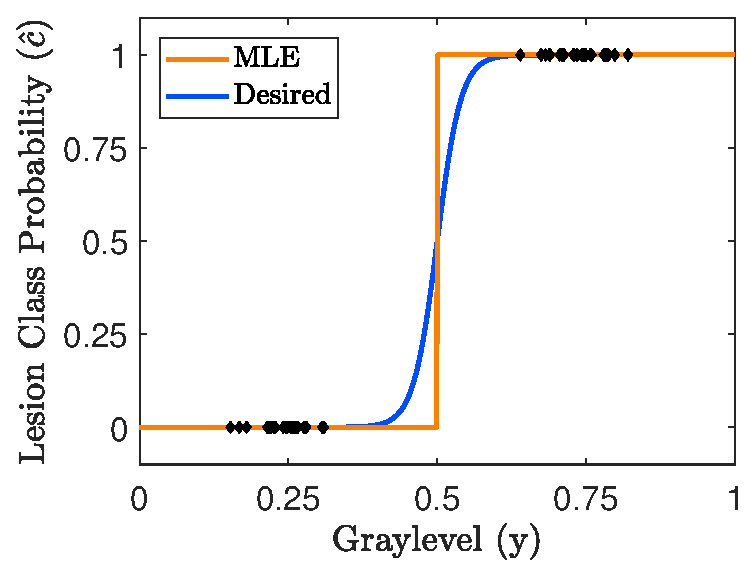
\includegraphics[width=\textwidth]{chmle-sep}
    \caption{Separable classes}%
    \label{fig:chmle-sep}
  \end{subfigure}
  \begin{subfigure}{\plotwidth}
    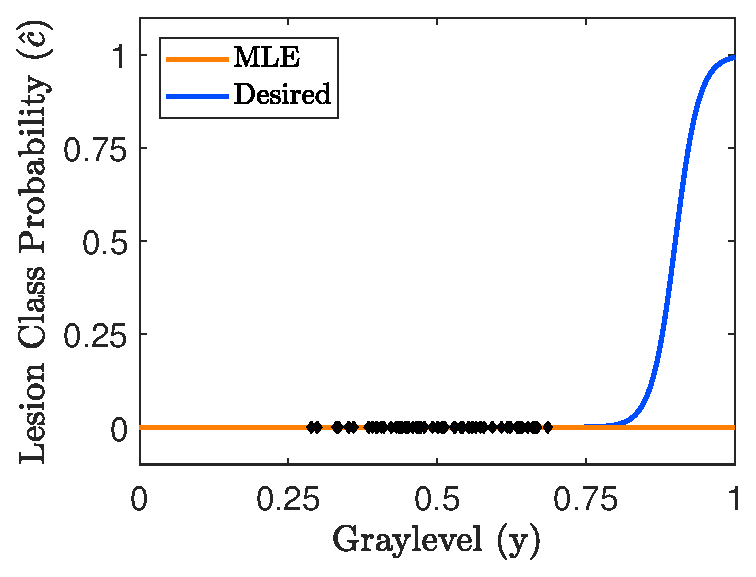
\includegraphics[width=\textwidth]{chmle-noles}
    \caption{No lesions}%
     \label{fig:chmle-noles}
   \end{subfigure}
  \caption{Challenges encountered during estimation of a logistic model.}%
  \label{fig:chmle}
\end{figure}
% ==================================================================================================
\subsection{Maximum Likelihood Estimation}
Each parameter vector $\bb(x)$ is considered completely independent.
Doing so greatly simplifies model fitting, but does not address the challenges described above.
These must instead be addressed using regularization strategies,
as discussed below in \S~\ref{s:vlr-reg}.
In this section, ML estimation of independent parameter vectors $\bb$ is developed.
For clarity, only a single voxel is considered -- i.e.\ $y$ from $Y(x)$, etc.
\par
As note above, the optimal $\bb$ for each independent voxel can be resolved using MLE.
If the training data are also assumed to be independently observed,
then the likelihood (conditioned on the data) is defined from binomial theory as
\begin{align}
  L(\bb\mid\C,\bY) &= \prod_{n=1}^{N} {P(c=1\mid\by_n;\bb)}^{c_n}
                              \left(1-{P(c=1\mid\by_n;\bb)}^{1-c_n}\right)\nonumber\\
                   &= \prod_{n=1}^{N} \Big[\hat{c}_n^{\en c_n}
                                   \left(1-\hat{c}_n^{\en 1-c_n}\right)\Big].%
  \label{eq:likelihood}
\end{align}
For computational reasons,
it is simpler and asymptotically equivalent to maximize the log-likelihood,
\begin{align}
  \L(\bb) &= \log{ \prod_{n=1}^{N} \Big[\hat{c}_n^{\en c_n}
                                \left(1-\hat{c}_n^{\en 1-c_n}\right)\Big] }\nonumber\\
          &= \sum_{n=1}^{N} \Big[ c_n \log \hat{c}_n + (1-c_n) \log (1-\hat{c}_n) \Big] \nonumber\\
          &= \sum_{n=1}^{N} \Big[ c_n \bb^T\by_n - \log (1+e^{\bb^T\by_n}) \Big].%
  \label{eq:loglikelihood}
\end{align}
The optimal $\bb$ is therefore resolved by maximizing the log-likelihood,
\begin{align}
  \bb^* &= \underset{\bb}{\arg\max}\en\L(\bb)\nonumber\\
        &= \underset{\bb}{\arg\max}\en\sum_{n=1}^{N}
             \Big[ c_n \bb^T\by_n - \log (1+e^{\et\bb^T\by_n}) \Big].%
  \label{eq:argmaxmle}
\end{align}
% ==================================================================================================
\subsection{Iterative Updates}
Estimation of $\bb^*$ can be performed using iterative optimization,
using an initial estimate $\bb^{(0)}$ and an update term $\Delta\bb^{(t)}$,
\begin{equation}
  \bb^{(t+1)} \leftarrow \bb^{(t)} + \alpha\thinspace\Delta\bb^{(t)},%
  \label{eq:update}
\end{equation}
where $\alpha$ is a small valued learning rate parameter.
There are many possible definitions of $\Delta\bb$,
including simply the gradient of $\L(\bb)$, denoted $\nabla_{\bb}\L$.
However, it can be shown that $\L(\bb)$ is convex, so higher order update equations can be used.
The work by~\citeauthor{Minka2003}~\cite{Minka2003} compares several options,
including Newton's method (and variants),
conjugate gradient, iterative scaling (and variants), and dual optimization.%
\footnote{Matlab code available at \hreftt{https://github.com/tminka/logreg/}}
For small feature dimensionality ($K$), performance differences among the options were small.
Classic Newton updates gave a good balance between memory requirements and computational order,
so they are used.
\par
If the gradient $\nabla_{\bb}\L$ and Hessian matrix $\nabla^2_{\bb}\L$ are defined as
\begin{align}
  \nabla_{\bb}\L   &= \left[\begin{array}{c}
                        \frac{\d L}{\d\b^1}\\\vdots\\\frac{\d L}{\d\b^\sk}
                      \end{array}\right],%
  \label{eq:llgradient0}\\
  \nabla^2_{\bb}\L &= \left[\begin{array}{ccc}
                        \frac{\d^2 L}{\d\b^1\d\b^1}   & \cdots & \frac{\d^2 L}{\d\b^1\d\b^\sk}\\
                                               \vdots & \ddots & \vdots \\
                        \frac{\d^2 L}{\d\b^\sk\d\b^1} & \cdots & \frac{\d^2 L}{\d\b^\sk\d\b^\sk}
                      \end{array}\right]%
  \label{eq:llhessian0},
\end{align}
then the Newton update is given by
\begin{equation}
  \Delta\bb = -{\nabla^2_{\bb}\L}^{-1}\nabla_{\bb}\L.%
  \label{eq:newtonmle}
\end{equation}
In the current model, the gradient is given by 
\begin{equation}
  \nabla_{\bb}\L = \sum_{n=1}^{N} \by_n\left(c_n - \hat{c}_n\right),%
  \label{eq:llgradient}
\end{equation}
and the Hessian by
\begin{equation}
  \nabla^2_{\bb}\L = \sum_{n=1}^{N} \by_n{\by_n}^T \left(c_n - \hat{c}_n\right).%
  \label{eq:llhessian}
\end{equation}
Substituting (\ref{eq:llgradient}) and (\ref{eq:llhessian}) into (\ref{eq:newtonmle}),
the explicit update $\Delta\bb$ for (\ref{eq:update}) is obtained.
At each iteration, $\Delta\bb^{(t)}$ is re-computed,
and the process continues until some convergence criterion is satisfied.
% ==================================================================================================
\subsection{Simplification}\label{ss:vlr-simple}
It is not necessary to complete the above procedure for all voxels in the standardized space.
Instead, only voxels in the expected location of the brain need to be computed;
such voxels can be selected using a binary ``brain mask'', denoted $M(x)$.
More details about the brain mask used in this work can be found in \S~\ref{ss:brainmask}.
Moreover, since the parameters of each voxel are estimated independently,
this can also be computed in parallel.
The details of this implementation are presented in \S~\ref{s:parallelfit},
after incorporation of the regularizations described in the next section.
\par
Finally, the model has so far been derived in general terms,
so that any choice of feature set $\by$ can be used.
However, with only one feature -- the FLAIR graylevel $y = y^1$ --
it is possible to reparameterize the sigmoid argument as
\begin{align}
  \bb^T\by &= \b^0(1) + \b^1(y)\nonumber\\
           &= s(y-\tau)
           \qquad\begin{cases}
             s = \b^1\\
             \tau = -\frac{\b^0}{\b^1}.
           \end{cases}%
  \label{eq:reparameterize}
\end{align}
In this form, the parameters $\tau$ and $s$ emerge
as a graylevel threshold and a slope parameter, respectively.
Specifically, when $y = \tau$,
the predicted probability of lesion is $\hat{c} = \tfrac{1}{1+e^{0}} = 0.5$,
so $\tau$ controls the location of the class discrimination,
as shown in Figure~\ref{fig:reparam-t}.
Similarly, the $s$ parameter defines the sensitivity of the logistic function to $y$,
as shown in Figure~\ref{fig:reparam-s}.
By contrast, varying the original parameter $\beta^1$ with $\beta^0$ constant
(Figure~\ref{fig:reparam-b1}) results in correlation of these characteristics.
These new parameters, and the corresponding images $\mathcal{T}(x)$ and $\mathcal{S}(x)$,
are therefore salient descriptors of the predictive model.
\begin{figure}
  \centering
  \begin{subfigure}{\plotwidth}
    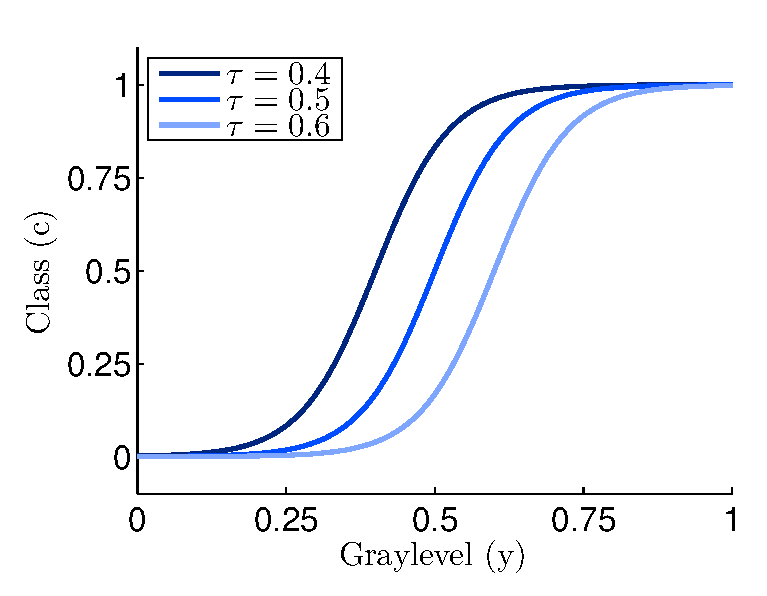
\includegraphics[width=\textwidth]{reparam-t}
    \caption{Vary $\tau$ with $s = 16$ constant.}%
    \label{fig:reparam-t}
  \end{subfigure}
  \begin{subfigure}{\plotwidth}
    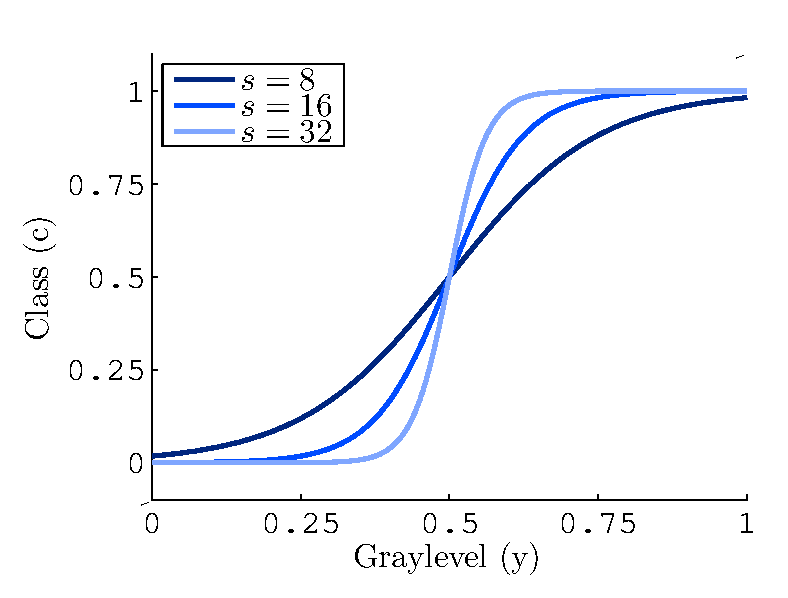
\includegraphics[width=\textwidth]{reparam-s}
    \caption{Vary $s$ with $\tau = 0.5$ constant.}%
    \label{fig:reparam-s}
  \end{subfigure}
  \begin{subfigure}{\plotwidth}
    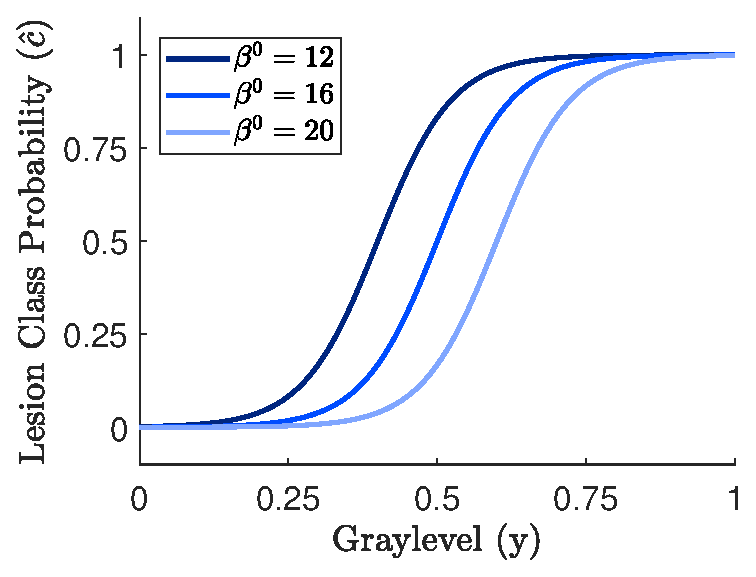
\includegraphics[width=\textwidth]{reparam-b0}
    \caption{Vary $\b^0$ with $\b^1 = 16$ constant.}%
    \label{fig:reparam-b0}
  \end{subfigure}
  \begin{subfigure}{\plotwidth}
    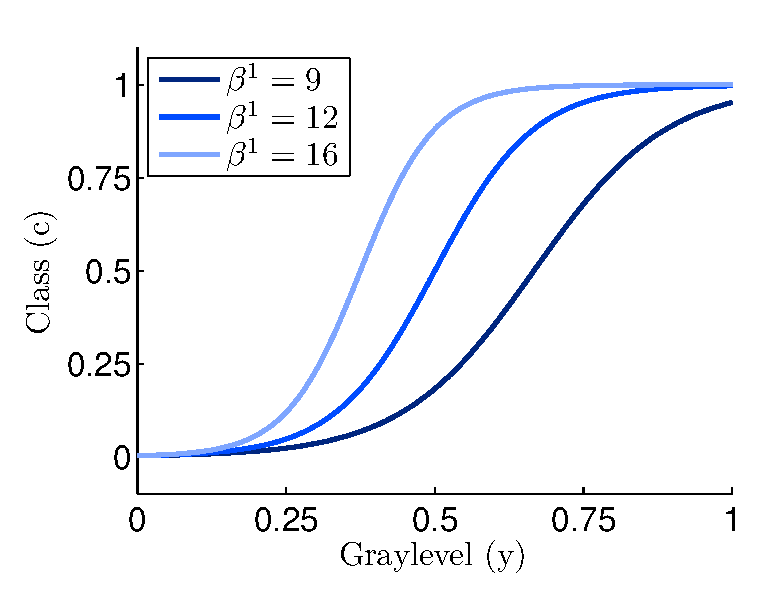
\includegraphics[width=\textwidth]{reparam-b1}
    \caption{Vary $\b^1$ with $\b^0 = -6$ constant.}%
    \label{fig:reparam-b1}
  \end{subfigure}
  \caption{Effect of varying the logistic model parameters.}%
  \label{fig:reparam}
\end{figure}
%%%%%%%%%%%%%%%%%%%%%%%%%%%%%%%%%%%%%%%%%%%%%%%%%%%%%%%%%%%%%%%%%%%%%%%%%%%%%%%%%%%%%%%%%%%%%%%%%%%%
\section{Regularization}\label{s:vlr-reg}
Regularizations are
methods of injecting prior knowledge about the expected model into the optimization.
Assuming voxel-wise independence of model parameters requires the use of regularization strategies
to solve the challenges outlined in \S~\ref{ss:modelfitting}.
Several regularization methods are explored below.
% ==================================================================================================
\subsection{Data Augmentation}\label{ss:vlr-reg-aug}
Noting the central role of training data in each of the challenges,
methods of artificially increasing the training dataset size
may be particularly useful in solving them.
Data augmentation has long been used in machine learning tasks with limited training data,
and there are several methods of generating synthetic data.
In low dimensional input/output spaces,
random sampling of fitted class-conditional posterior distributions
can produce reasonable samples with known labels~\cite{Tanner1987}.
In higher dimensional problem spaces, however, imputation is more difficult~\cite{Goodfellow2014}.
For example, the space of potential $100\times100\times100$-sized images has $100^3$ dimensions
(one per voxel), yet only a small subspace represents plausible images.
Generating synthetic examples in this space is therefore challenging,
especially for segmentation tasks,
where the outputs have dimensionality roughly equal to the input.
\par
Alternatively, simple image manipulations can still afford model improvements~\cite{Krizhevsky2012}.
In segmentation tasks, both the input image(s) and the corresponding label images can be
translated, reflected, rotated, and perhaps resized,
thereby avoiding the generation of genuinely synthetic examples.
In the current work, reflections and small (one-voxel) translations
can be applied to the label and FLAIR images following registration to the MNI brainspace.
The potential benefits of this augmentation are explored in \S~\ref{ss:exp-reg}.
%__JK__ need also to define MNI before here...?
% ==================================================================================================
\subsection{Classic Regularization}\label{ss:vlr-reg-lambda}
The separable classes challenge is well-known in regression problems,
and a good solution is to penalize the magnitude of model parameters using the $L_p$-norm:
$\lambda\norm{\bb}_p$~\cite{Zou2005}.
It can be shown that $L_1$ regularization corresponds to a Laplacian prior on elements of $\bb$,
with scale parameter inversely proportional to $\lambda$
(equivalently, this assumes that the model error follows this distribution).
Similarly, $L_2$ regularization implies a Gaussian prior,
with standard deviation inversely proportional to $\lambda$~\cite{Zou2005}.
Model fitting which includes this prior-derived term is called
maximum a posteriori (MAP) estimation,
and the penalty can be appended to the objective function (\ref{eq:argmaxmle}), as in
\begin{align}
  \bb^* &= \underset{\bb}{\arg\max}\en\J(\bb) \nonumber\\
        &= \underset{\bb}{\arg\max}\en\L(\bb) - \lambda\norm{\bb}_p \nonumber\\
        &= \underset{\bb}{\arg\max}\en\sum_{n=1}^{N}
           \Big[ c_n \bb^T\by_n - \log (1+e^{\et\bb^T\by_n}) \Big] - \lambda\norm{\bb}_p.%
  \label{eq:argmaxmap}
\end{align}
Due to its relatively large gradient near zero,
$L_1$ regularization is typically used to encourage sparsity in the feature weights
(i.e.\ $\b^k\rightarrow0$)~\cite{Tibshirani1996}.
This is not desirable in the current model,
since the feature (FLAIR graylevel) is known to be discriminative.
Moreover, the expansion of the $\norm{\bb}_1$ term
in the gradient of the objective function is not straightforward,
since it is non-differentiable at zero~\cite{Tibshirani1996,Lee2006}.
Conversely, $L_2$ regularization is more effective at limiting parameter magnitude
-- which is the current aim --
and the first and second order gradients of (\ref{eq:argmaxmap}) derive easily~\cite{Minka2003}.
For these reasons, only $L_2$ regularization is considered,
yielding the following change to the Newton update expression (\ref{eq:newtonmle}),
\begin{align}
  \Delta\bb&=-{\nabla^2_{\bb}\J}^{-1}\nabla_{\bb}\J \nonumber\\
           &=-{\left(\nabla^2_{\bb}\L-\lambda I\right)}^{-1}\left(\nabla_{\bb}\L-\lambda\bb\right).%
  \label{eq:newtonmap}
\end{align}
What remains is to select an appropriate value of $\lambda$.
This is explored experimentally in \S~\ref{ss:exp-toy-lam} using a toy model.
% ==================================================================================================
\subsection{Pseudo-Lesions}\label{ss:vlr-reg-pseudo}
The sparsely observed lesion class challenge is less common,
since discriminative models are rarely fit in the absence of one class altogether.
This occurs here because all voxels are modelled independently.
It is therefore tempting to simply sample features from the lesion class at other spatial locations
in order to fit the logistic model in the healthy training voxels,
similar to the approach by~\citeauthor{Schmidt2017a}.
However, as noted in \S~\ref{ss:autochallenges} and \S~\ref{sss:limits-flair},
WML are thought to have different intensities
in different brain regions~\cite{Stevenson2000,Sled2004},
and some locations will likely never contain any WMH.
Considering these facts, the use of deterministic synthetic lesion-class samples,
or ``pseudo-lesions'', could instead permit better use of prior knowledge about WMH.
These synthetic observations could be appended to the training data for each voxel
so as to minimally balance the training classes,
and act as a prior on the distribution of lesion-class features.
% This approach would not be subject to variations in the training data,
% and it would be feasible to consider the prior probability of healthy tissues
% (GM / WM / CSF) in the definition.
\par
If the same number of synthetic observations are appended to the training data for each voxel,
this is equivalent to appending a number of synthetic images to the training set.
The synthetic feature data are denoted
$\bV(x) = \{\bm{\gamma}_{1}(x),\dots,\bm{\gamma}_{\sv}(x)\}$.
It is assumed that the labels of all synthetic data are ``lesion'',
so the set of synthetic label images is simply denoted $\bm{1}(x)$.
The updated training set is therefore
$\bY_{\gamma}(x) = \{\bY(x),\bV(x)\}$, and $\bC_{\gamma}(x) = \{\bC(x),\bm{1}(x)\}$.
\par
Design of the synthetic image set $\bV(x)$ should be guided by prior knowledge.
For the same reasons as described above,
it is not possible to derive this knowledge from the training set.
Unfortunately, few other sources of structured information are available.
One reasonable approach could make use of healthy tissue prior probability images
(Figure~\ref{fig:tpm-3}), denoted $\rho(x)$.
Specifically, the expected intensity for the lesion class in each tissue
can be multiplied by the tissue probability image,
and the results summed to give the overall synthetic image,
\begin{equation}
  \gamma(x) = \gamma_{\gm{}}\cdot\rho_{\gm{}}(x)
            + \gamma_{\wm{}}\cdot\rho_{\wm{}}(x)
            + \gamma_{\csf{}}\cdot\rho_{\csf{}}(x).
\end{equation}
While WMH are not possible in either the GM or the CSF,
it is necessary to select a FLAIR graylevel
-- perhaps the maximum possible intensity --
to complete this model.
Additionally, such parameters will inevitably play a role
for subjects with imperfect registration or outlier anatomy.
The contributions of pseudo-lesions to model fitting
are explored experimentally in \S~\ref{ss:exp-toy-psu}.
%__JK__ should TPMs be introduced sooner?
\begin{figure}
  \centering
  \subfigureoverl[white]{(a) $\rho_{\gm{}}(x)$}{}{%
    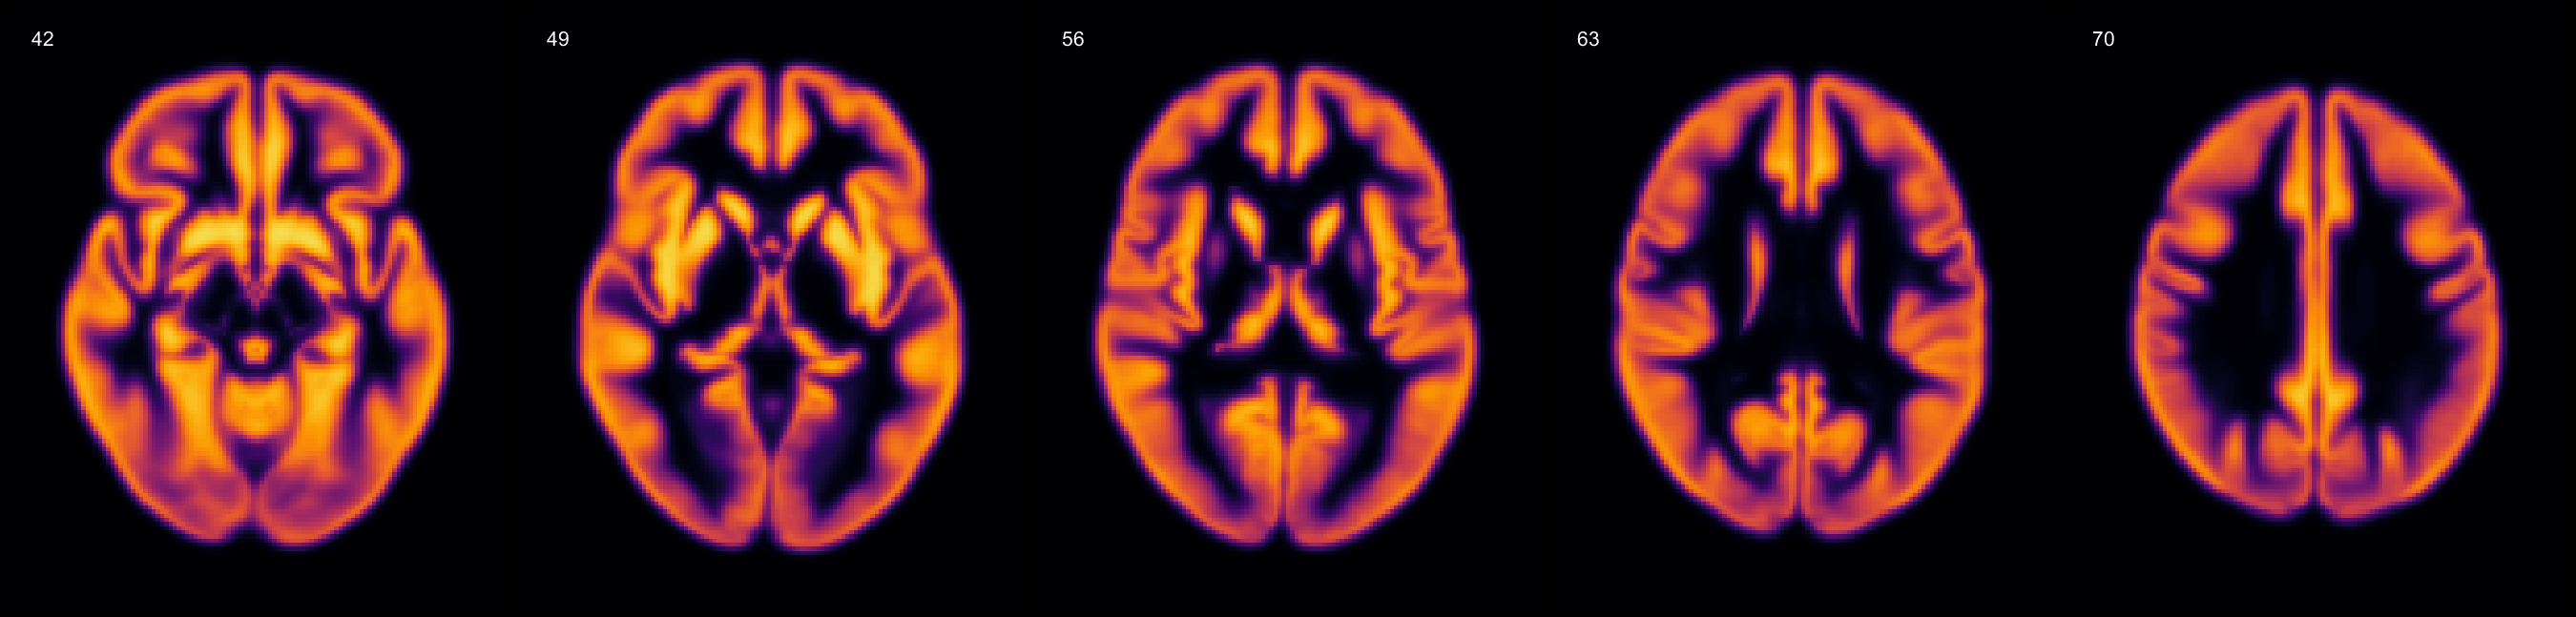
\includegraphics[height=\sliceheight]{tpm-gm.png}
    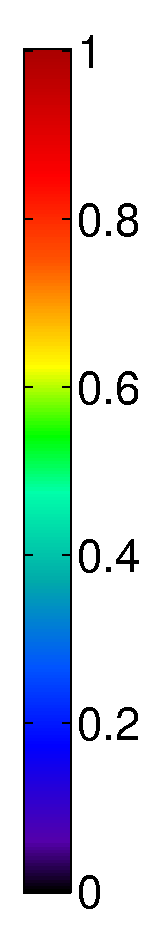
\includegraphics[height=\sliceheight]{cmap-tpm}%
  }\\[0.5em]
  \subfigureoverl[white]{(b) $\rho_{\wm{}}(x)$}{}{%
    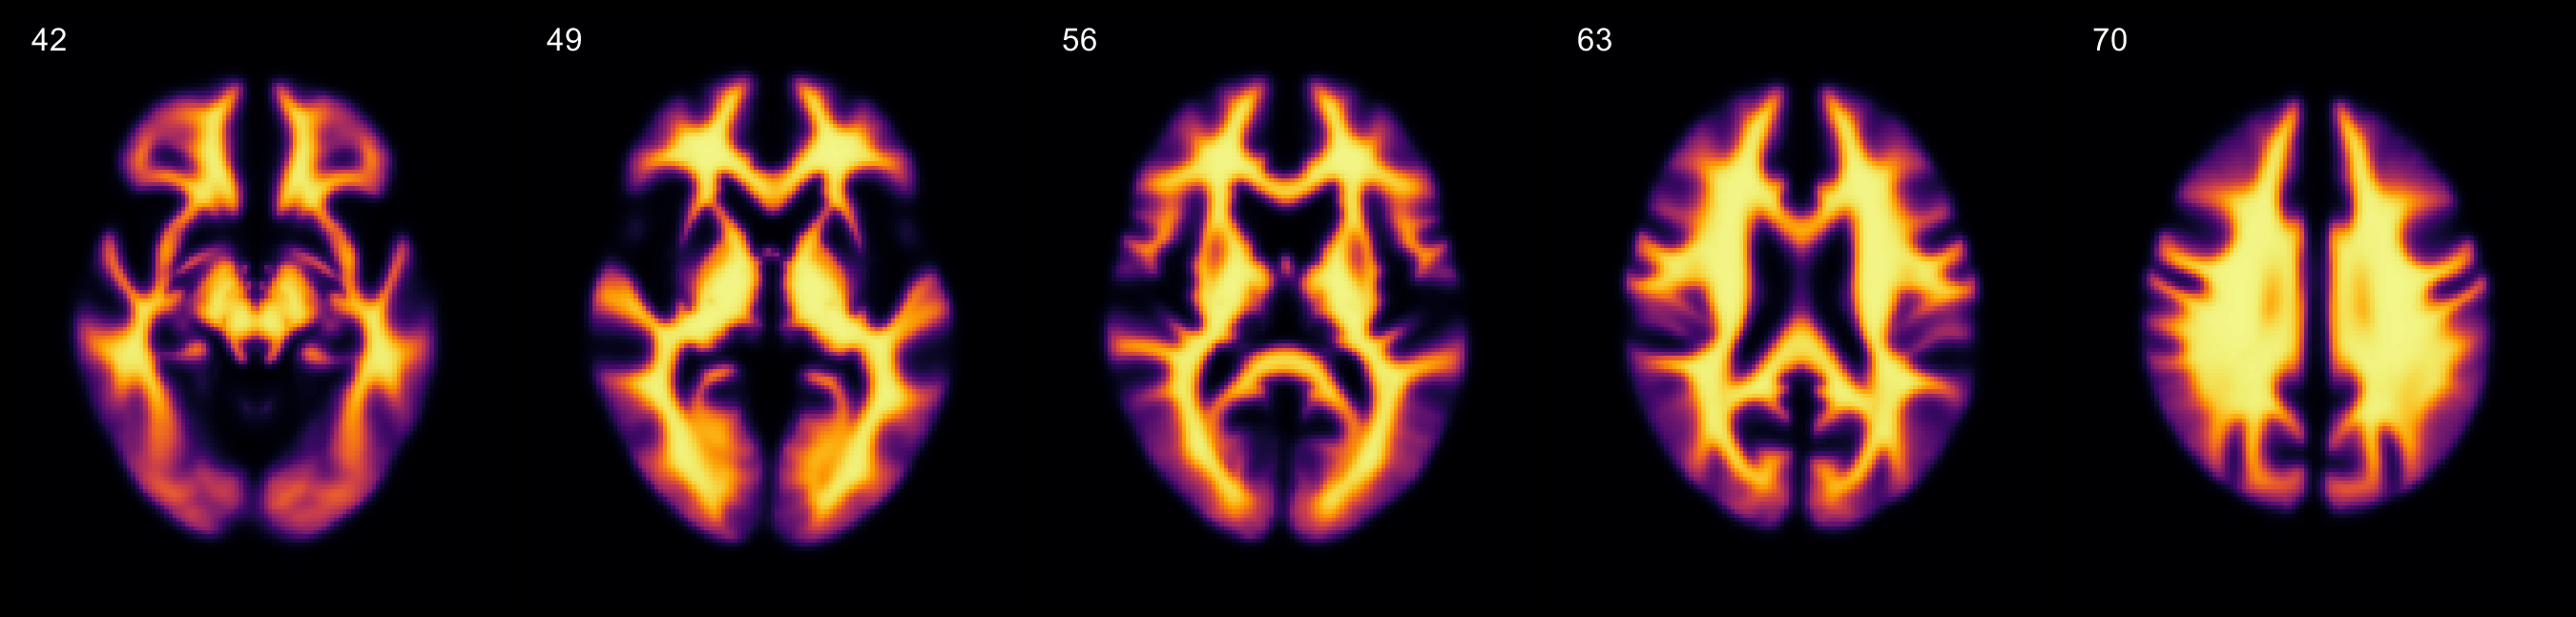
\includegraphics[height=\sliceheight]{tpm-wm.png}
    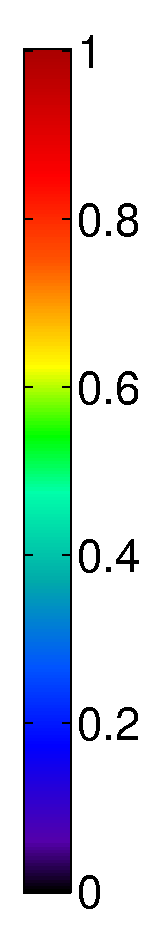
\includegraphics[height=\sliceheight]{cmap-tpm}%
  }\\[0.5em]
  \subfigureoverl[white]{(c) $\rho_{\csf{}}(x)$}{}{%
    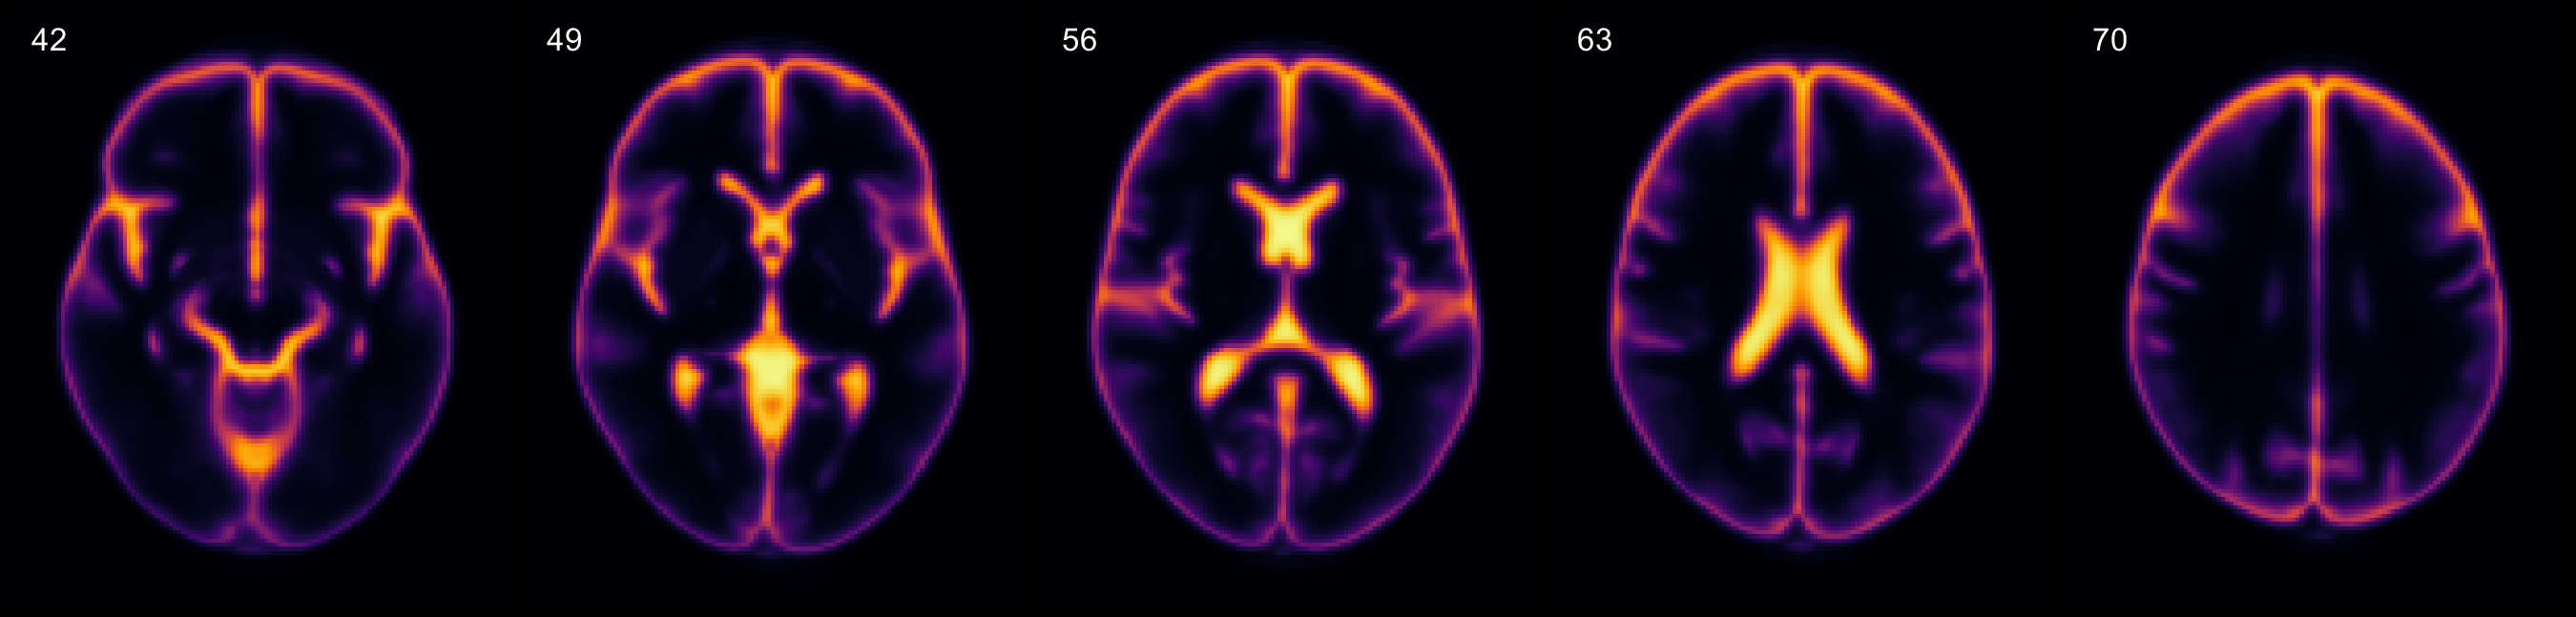
\includegraphics[height=\sliceheight]{tpm-csf.png}
    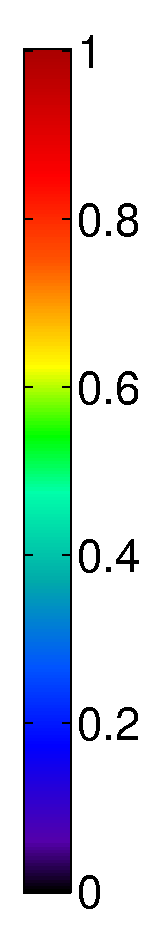
\includegraphics[height=\sliceheight]{cmap-tpm}%
  }
  \caption{Tissue prior probability images in MNI space.
    Derived from~\cite{Mazziotta2001}. Best viewed in colour.}%
  \label{fig:tpm-3}
\end{figure}
% ==================================================================================================
\subsection{Parameter Image Smoothing}\label{ss:vlr-reg-smooth}
Finally, independent model fitting in every voxel risks yielding noisy parameter images.
The simplest solution to this problem involves
filtering the reconstructed parameter images after estimation.
A wide range of possible filters for this task exist,
and a selection of these are summarized in Table~\ref{tab:filters},
including the mutable parameters for each.
\begin{table}
  \centering
  \caption{Image filters considered for smoothing the estimated parameter images.}%
  \label{tab:filters}
  \begin{tabular}{llllc}
  	\toprule
  	Name      & Parameters            & Advantages                   & Disadvantages    &        Ref.         \\ \midrule
  	Gaussian  & width $\sigma$        & no artifacts                 & blurs edges      & \cite{Gonzalez2006} \\ % chktex 2
  	Median    & width $w$             & preserves edges              & square artifacts & \cite{Gonzalez2006} \\ % chktex 2
  	Bilateral & $\sigma_y$,$\sigma_x$ & balanced blurring and detail & Expensive        &  \cite{Tomasi1998}  \\ \bottomrule % chktex 2
  \end{tabular}
\end{table}
\par
An alternative solution might involve modelling the parameter images as a spatial function
(e.g.\ band-limited discrete cosine / Fourier transform).
However, there are two challenges with this approach.
First, deriving the update gradients for such a model would be challenging,
and their computation could significantly increase training time.
Second, such an encoding may introduce artifacts in the resulting parameter images.
Moreover, it is well known that frequency domain band-limiting
can be equivalently achieved by convolution (i.e.\ filtering)
in the spatial domain~\cite{Gonzalez2006}.
Therefore, only conventional filtering is explored in this work (cf.~\S~\ref{ss:exp-beta}).
%__JK__ define this reference in ch-exp
%__JK__ address MRFs for smoothing here?
%%%%%%%%%%%%%%%%%%%%%%%%%%%%%%%%%%%%%%%%%%%%%%%%%%%%%%%%%%%%%%%%%%%%%%%%%%%%%%%%%%%%%%%%%%%%%%%%%%%%
\section{Post-Processing}\label{s:vlr-post}
At this point, the motivation and details of the proposed VLR model have been presented,
in addition to the preprocessing steps required to satisfy its assumptions.
The last component of a segmentation pipeline typically includes post-processing. 
In principle, this step aims to incorporate any additional knowledge of the problem
which has not been considered in upstream elements.
Here, these include the connected morphology of WML, and the minimum lesion size.
Discussions of these topics, however, would assume that the label image is already binary,
whereas the output from the VLR model is probabilistic.
Therefore, the first post-processing step
thresholds the WMH class probability at a value $\pi$ to give a ``hard'' classification:
$\hat{c}\rightarrow \hat{c}^{\pi}$
This also facilitates comparison with manual segmentation masks, which are usually binary.
% ==================================================================================================
\subsection{Thresholding}\label{ss:vlr-thr}
If the assumptions of any probabilistic model are valid,
then the ``hard'' classification between any set of classes $c$ is straightforward:
\begin{equation}
  \hat{c}^{\pi} = \underset{c}{\arg\max}\en p(c\mid\by;\bb).
\end{equation}
In a 2-class logistic regression model, this simplifies to thresholding at $p$:
\begin{equation}
  \hat{c}^{\pi} = \begin{cases} 0 & \hat{c} < \pi \\ 1 & \hat{c} \ge \pi, \end{cases}
\end{equation}
with $\pi = 0.5$.
However, since these assumptions are often only partially true,
most models are able to achieve better agreement with manual segmentations
using a different threshold $\pi$ for the WMH class.
In fact several of the freely available toolboxes% (cf.~\S~\ref{sss:wmhsegtoolboxes})
permit a user-specified threshold which can be optimized for the user's data.
During model validation,
this parameter should be optimized using the training data for each cross validation fold.
It is also prudent to illustrate the sensitivity of the model to this parameter, using either 
a plot of performance versus threshold~\cite{Steenwijk2013}, or
a precision-recall (PR) curve~\cite{Arbelaez2011}.
In the current work, both these techniques are employed:
$\pi$ is optimized on the fly, and a PR curve is given after.
% ==================================================================================================
\subsection{Minimum Lesion Size}\label{ss:vlr-minx}
With finite image resolution and appreciable noise in MRI,
lesions appearing as only a few connected voxels are indistinguishable from image noise,
even by human experts.
Such potential lesions are therefore not included in radiologists assessment of WML.
Accordingly, most WMH segmentation algorithms employ
a minimum-connected-voxels exclusion criterion during post-processing.
Connectedness can be defined in 2D or 3D,
and consider only direct adjacency or diagonal connections too.
Most works employ the most liberal definition: 26-connectedness,
which considers all $3\times3\times3-1=26$ candidates surrounding a given voxel in 3D.
Ideally, the number of required connected voxels will adapt to the image resolution,
and correspond to a minimum lesion volume.
Typical volumes range from about $\mathrm{x}_{\min}^{c} = $
$3.5$ mm\textsuperscript{3} in~\cite{Steenwijk2013,Fartaria2015}, to 
$9.0$ mm\textsuperscript{3} in~\cite{Yoo2014,Elliott2013}.
\par
In the current work, the inclusion of a minimum lesion size rule is explored.
The optimal value for $\mathrm{x}_{\min}^{c}$ is resolved experimentally
during each cross validation fold, and the resulting values compared with the above conventions.
Additionally, the gains in performance afforded by this step are quantified.
% __JK__ I was going to include the MRF in this section too,
% but since I really didn't investigate these in any great detail,
% I was hoping to omit this overall. I would save a lot of time running experiments,
% and also they never seemed to improve performance (in fact, the opposite).
% It would require a lot more tinkering to get some good results,
% and I don't think I'm really in that position right now.
% __JK__
% \subsection{Connected Morphology of WML}
% \par...\par
% Preliminary qualitative investigations into lesions with these characteristics
% suggested that errors in this area were not a significant problem for the model.
%%%%%%%%%%%%%%%%%%%%%%%%%%%%%%%%%%%%%%%%%%%%%%%%%%%%%%%%%%%%%%%%%%%%%%%%%%%%%%%%%%%%%%%%%%%%%%%%%%%%
% __JK__ what to do about this ugly \hat{c}^{\circ} notation from above?
%        Keep for all references to the hard labelled images? :(
%%%%%%%%%%%%%%%%%%%%%%%%%%%%%%%%%%%%%%%%%%%%%%%%%%%%%%%%%%%%%%%%%%%%%%%%%%%%%%%%%%%%%%%%%%%%%%%%%%%%
\section{Model Summary}
In summary, the proposed algorithm uses graylevel features
to train a logistic regression model for each voxel independently -- Voxel-Wise Logistic Regression.
In order to train the VLR model,
a set of labelled training images must first be registered to a standard brain space (MNI).
This is achieved using the SPM Segment tool, which also produces bias corrected images.
Next, image intensities are standardized using a graylevel transformation,
to be determined in the next section.
The parameter images $\bb(x)$ are then computed using iterative MAP estimation,
with Newton updates and an augmented dataset.
These images are smoothed to reflect prior knowledge.
Finally, the optimal probability threshold $\pi$
and minimum lesion size $\mathrm{x}_{\min}^{c}$
are estimated using the training data.
This completes the training phase.
\par
At test time, SPM Segment is used again to
correct the bias field and estimate the registration to MNI space for a given input image.
However, the inverse transform is now used to warp the parameter images $\bb(x)$
from MNI space to the native space.
This transformation of the smooth parameter images prior to inference is preferable
to transforming the detailed label image afterwards.
The probability of the WMH class is computed
by evaluating the independent logistic models at every voxel.
This initial estimate $\hat{C}(x)$ is then thresholded using $\pi$,
and binary objects smaller than $\mathrm{x}_{\min}^{c}$ are removed.
The resulting label image is the final output.
These training and testing phases are illustrated in Figure~\ref{fig:modelsum}.
\begin{figure}
  \centering\scalebox{0.65}{\pgfdeclarelayer{background}
\pgfdeclarelayer{foreground}
\pgfsetlayers{background,main,foreground}
\tikzset{%
  arrow/.style = { ->, >=Latex,  very thick, rounded corners, draw = #1!60!white },
  input/.style = { ->, >=Latex, ultra thick, rounded corners, draw = red },
  clr/.style   = { ultra thick, rounded corners, fill = #1!60!white },
  image/.style = { fill = black, draw = black!80!white, ultra thick, inner sep = 0 },
  plot/.style  = { fill = white, inner sep = 0 },
  label/.style = { fill = white, fill opacity = 0, text opacity = 1 },
  tbox/.style  = { fill = white, draw = #1!60!white, very thick, align = center }
}
\newcommand*{\img}[3]{%
  \node[image] at (#1,#2){\includegraphics[width=\ixx cm, height=\iyy cm]{#3}}; % chktex 1
}
\newcommand*{\imgt}[4]{%
	\img{#1}{#2}{#3}
	\begin{pgfonlayer}{foreground}
		\node[label] at (#1,#2-\iy-0.4){\large #4};
	\end{pgfonlayer}
}
\newcommand*{\plot}[5]{%
  \node[plot] at (#1,#2){\includegraphics[width=#3cm, height=#4cm]{#5}};
}
\newcommand*{\voxpath}[4]{%
  \filldraw[fill=black!20!white,draw=black]
  (#1,#2)--(#1+\vw,#2)--(#1+#3,#2-#3+\vw)--(#1+#3-\vw,#2-#3+\vw)--(#1,#2);
  \filldraw[fill=black!20!white,draw=black]
  (#1,#2)--(#1,#2-\vw)--(#1+#3-\vw,#2-#3)--(#1+#3-\vw,#2-#3+\vw)--(#1,#2);
  \filldraw[fill=black!20!white,draw=black]
  (#1+#3,#2-#3)--(#1+#3,#2-#3+\vw)--(#1+#3-\vw,#2-#3+\vw)--(#1+#3-\vw,#2-#3)--(#1+#3,#2-#3);
  \node[below right] at (#1+#3,#2-#3) {#4};
}
\newcommand*{\imgstack}[5]{%
  \foreach \x in {0,...,#3}{\img{#1-0.1*#3+0.1*\x}{#2+0.1*#3-0.1*\x}{#4}} % chktex 11 chktex 1
  \begin{pgfonlayer}{foreground}
	  \node[label] at (#1,#2-\iy-0.4){\large #5};
	\end{pgfonlayer}{foreground}
}
\newcommand*{\imgvoxstack}[5]{%
	\voxpath{#1+\vw+0.3-0.1*#3-\vl-\vl}
					{#2-\vw-0.2+0.1*#3+\vl+\vl}{\vl}{}
	\imgstack{#1}{#2}{#3}{#4}{#5}
	\voxpath{#1+\vw+0.3}
	        {#2-\vw-0.2}{\vl}{}
}
\newcommand*{\textbox}[6]{%
  \node[tbox=#5,minimum width=#3cm,minimum height=#4cm]at(#1,#2){#6};
}
%\newcommand*{\blocktitle}[4]{%
%  \node[title=#3]at(#1,#2){#4};
%  \fill[clr=#3](#1+0.6,#2+1.7)--(#1+0.6,#2-1.7)--(#1+0.6+0.3,#2);
%}
\newcommand*{\vw}{0.1}
\newcommand*{\vl}{0.7}
\newcommand*{\ix}{0.8}\newcommand*{\ixx}{1.6}
\newcommand*{\iy}{1}  \newcommand*{\iyy}{2}
\newcommand*{\pw}{1.5}
\newcommand*{\fw}{0.3}

% --------------------------------------------------------------------------------------------------
\begin{tikzpicture}
    \useasboundingbox(1.5, 0.0) rectangle (24.0, 20.5);
    \begin{pgfonlayer}{background}
      % background boxes
      \draw[black!30!white,rounded corners,very thick](-0.25, 0.25) rectangle (23.75, 9.75);
      \draw[black!30!white,rounded corners,very thick](-0.25,10.25) rectangle (23.75,20.00);
      % box labells
      \node[fill=black!10!white,rounded corners,minimum width=3cm, minimum height=1.0cm]
        at(21.75,19.00){\textsc{Training}};
      \node[fill=black!10!white,rounded corners,minimum width=3cm, minimum height=1.0cm]
        at(21.75, 8.75){\textsc{Testing}};
      %\draw[step=0.5,black!10!white,very thin](-0.5, 0.0) grid (24.0,20.0);
    \end{pgfonlayer}
    % training
    \imgt       { 1.0}{18.0}{c1}{$\mathrm{C}_1(x)$}
    \imgt       { 1.0}{14.0}{c2}{$\mathrm{C}_{\textsc{n}}(x)$}
    \imgt       { 3.0}{18.0}{i1}{$\mathrm{Y}_1(x)$}
    \imgt       { 3.0}{14.0}{i2}{$\mathrm{Y}_{\textsc{n}}(x)$}
    \node[font=\fontsize{30}{0}\selectfont,align=center] at ( 1.0,15.8) {$\vdots$};
    \node[font=\fontsize{30}{0}\selectfont,align=center] at ( 3.0,15.8) {$\vdots$};
    \imgstack   {10.0}{16.0}{6}{ir} {$\mathcal{Y}(x)$}
    \imgvoxstack{13.0}{16.0}{6}{jr} {$\tilde{\mathcal{Y}}(x)$}
    \imgvoxstack{13.0}{12.0}{6}{c1} {$\mathcal{C}(x)$}
    \plot       {17.5}{14.0}{4}{4}  {lr-fit}
    \imgvoxstack{22.0}{14.0}{1}{bb} {$\bm{\beta}(x)$}
    % testing
    \imgstack   { 3.0}{ 2.0}{1}{bb} {$\bm{\beta}(x)$}
    \imgvoxstack{ 3.0}{ 6.0}{0}{it} {$Y_{test}(x)$}
    \imgvoxstack{10.0}{ 2.0}{1}{bb} {$\bm{\upbeta}(x)$}
    \imgvoxstack{10.0}{ 6.0}{0}{jt} {$\tilde{\mathrm{Y}}_{test}(x)$}
    \plot       {14.5}{ 4.0}{4}{4}  {lr-test}
    \imgvoxstack{19.0}{ 4.0}{0}{qt} {$\hat{\mathrm{C}}_{test}(x)$}
    \imgt       {22.0}{ 4.0}{lt}    {$\hat{\mathrm{C}}_{test}^{\circ}(x)$}
    % training arrows
    \draw[arrow={blue}  ]( 3.0+\ix,18.0    )--( 3.5+\ix,18.0)--( 3.5+\ix,16.0)--( 5.0,16.0);
    \draw[arrow={blue}  ]( 3.0+\ix,16.0    )--( 5.0    ,16.0);
    \draw[arrow={blue}  ]( 3.0+\ix,14.0    )--( 3.5+\ix,14.0)--( 3.5+\ix,16.0)--( 5.0,16.0);
    \draw[arrow={blue}  ]( 8.0    ,16.0    )--(10.0-\ix,16.0);
    \draw[arrow={blue}  ]( 1.0    ,12.3    )--( 1.0    ,12.0)--( 5.0,    12.0);
    \draw[arrow={blue}  ]( 5.0    ,12.0    )--(13.0-\ix,12.0);
    \draw[arrow={blue},dotted](6.5,16.0    )--( 6.5    ,12.5);
    \draw[arrow={violet}](10.0    ,16.0+\iy)--(10.0    ,18.5);
    \draw[arrow={violet}](11.5,    19.0    )--(13.0    ,19.0)--(13.0,16.0+\iy);
    \draw[arrow={red}   ](13.0+\ix,16.0    )--(14.5    ,16.0)--(14.5,14.0)--(15.5,14.0);
    \draw[arrow={red}   ](13.0+\ix,12.0    )--(14.5    ,12.0)--(14.5,14.0)--(15.5,14.0);
    \draw[arrow={red}   ](19.5    ,14.0    )--(22.0-\ix,14.0);
    % testing arrows
    \draw[arrow={blue}  ]( 3.0+\ix, 6.0    )--( 5.0    , 6.0);
    \draw[arrow={blue},dotted](6.5, 6.0    )--( 6.5    , 2.5);
    \draw[arrow={blue}  ]( 3.0+\ix, 2.0    )--( 5.0    , 2.0);
    \draw[arrow={blue}  ]( 8.0    , 2.0    )--(10.0-\ix, 2.0);
    \draw[arrow={violet}]( 6.5    , 6.5    )--( 6.5    , 8.0);
    \draw[arrow={violet}]( 8.0    , 8.5    )--(10.0    , 8.5)--(10.0    , 6.0+\iy);
    \draw[arrow={red}   ](10.0+\ix, 6.0    )--(11.5    , 6.0)--(11.5, 4.0)--(12.5, 4.0);
    \draw[arrow={red}   ](10.0+\ix, 2.0    )--(11.5    , 2.0)--(11.5, 4.0)--(12.5, 4.0);
    \draw[arrow={red}   ](16.5    , 4.0    )--(19.0-\ix, 4.0);
    \draw[arrow={orange}](19.0    , 4.0+\iy)--(19.0    , 6.5);
    \draw[arrow={orange}](20.5,     7.0    )--(22.0    , 7.0)--(22.0, 4.0+\iy);
    % training texts
    \textbox    { 6.5}{16.0}{3}{1.0}{blue}  {Bias Correction\\\& Registration}
    \textbox    { 6.5}{12.0}{3}{1.0}{blue}  {Same Transform\\Applied}
    \textbox    {10.0}{19.0}{3}{1.0}{violet}{Histogram\\Matching}
    \textbox    {17.5}{17.0}{4}{1.0}{red}   {Logistic Regression\\Model Fitting}
    % testing texts
    \textbox    { 6.5}{6.25}{3}{0.5}{blue}  {Bias Correction}
    \textbox    { 6.5}{5.75}{3}{0.5}{blue}  {Registration}
    \textbox    { 6.5}{ 2.0}{3}{1.0}{blue}  {Inverse Transform\\Applied}
    \textbox    { 6.5}{ 8.5}{3}{1.0}{violet}{Histogram\\Matching}
    \textbox    {14.5}{ 7.0}{4}{1.0}{red}   {Logistic Regression\\Lesion Prediction}
    \textbox    {19.0}{ 7.0}{3}{1.0}{orange}{Post\\Processing}
\end{tikzpicture}}
  \caption{Overview of the proposed algorithm.
    Typefaces --
    upright Roman: images in native space;
    italic Roman: images in standard (MNI) space;
    calligraphic: a set of images from several patients;
    bold: a set of images corresponding to different features;
    Variables --
    $C(x)$: manual segmentation;
    $Y(x)$: FLAIR image;
    $\beta(x)$: parameter image;
    $\hat{C}(x)$: estimated lesion segmentation.
    Best viewed in colour.}%
  \label{fig:modelsum}
\end{figure}
% ==================================================================================================
\subsection{Tunable Parameters}
In order to achieve the best possible model performance,
it is prudent to track tunable model parameters (\textsc{aka} hyperparameters)
which are distinct from those fitted during each cross validation fold
-- i.e.\ $\bb(x)$ and $\pi$.
Considering both the main VLR model and the pre- and post-processing aspects,
the parameters of the proposed algorithm are summarized in Table~\ref{tab:hyp-base}.
%and also programmatically in \nameref{m:hypdef.m}.
The optimization of these model components will be the subject of the next chapter.
\begin{table}
  \centering
  \caption{Model hyperparameters and baseline values.}%
 \label{tab:hyp-base}
  \begin{tabular}{llccc}
  	\toprule
  	Stage                            & Parameter              &         Notation          &            Type            &         Baseline          \\ \midrule
  	\multirow{4}{*}{Pre-Processing}  & Reflect Augmentation   & $\mathrm{a}_{\textsc{r}}$ &        $\mathbb{B}$        &         \false{}          \\
  	                                 & Shift Augmentation     & $\mathrm{a}_{\textsc{s}}$ &       $\mathbf{N}_p$       &      $\mathbf{N}_0$       \\
  	                                 & Graylevel Transform    &        $\uptau_y$         &     $f: \Re\mapsto\Re$     &  $\uptau_{\textbf{RM3}}$  \\
  	                                 & Transform Mask         &       $\X_{\uptau}$       &      $\mathbb{B}(x)$       &    $\X_{\text{brain}}$    \\ \midrule
  	\multirow{7}{*}{VLR Fitting}     & Iterations             &            $T$            &        $\mathbb{Z}$        &           $30$            \\
  	                                 & Initial $\bb$          &        $\bb^{(0)}$        &          $\Re^2$           &          $[0,0]$          \\
  	                                 & Estimation Scale\ss{a} &       $\mathrm{r}$        &           $\Re$            &           $0.5$           \\
  	                                 & Learning Rate          &         $\alpha$          &           $\Re$            &            $1$            \\
  	                                 & Regularization         &         $\lambda$         &           $\Re$            &            $0$            \\
  	                                 & Pseudo-Lesions         &         $\bV(x)$          &    $\{\et\cdot\in\Re\}$    &          $\{\}$           \\
  	                                 & $\bb$ Filter           &         $F_{\bb}$         & $f: \Re(x) \mapsto \Re(x)$ & $\tilde{\bb}(x) = \bb(x)$ \\ \midrule
  	\multirow{1}{*}{Post-Processing} & Min Lesion  Size       &  $\mathrm{x}_{\min}^{c}$  &  $\Re\en(\text{mm}^{3})$   &            $0$            \\ \bottomrule
  	%                                & MRF Iterations         &      $N_{t}^{\mrf}$       &        $\mathbb{Z}$        &            $0$            \\
  	%                                & MRF Weights            &        $W_{\mrf}$         & $\{w_{\Delta},w_{F},w_y\}$ &        $\{1,1,1\}$
  \end{tabular}
  \tablepost{Notation.
    $\mathbb{B}$: boolean value;
    $\mathbb{Z}$: integer value;
    $\Re$: real value;
    $\Re^n$: vector;
    $\Re(x)$: image;
    $\mathbf{N}_p$: nearest $p$ voxel neighbourhood.
  \ss{a} cf.~\S~\ref{ss:halfres}.}
\end{table}
% --------------------------------------------------------------------------------------------------
% ==================================================================================================
%%%%%%%%%%%%%%%%%%%%%%%%%%%%%%%%%%%%%%%%%%%%%%%%%%%%%%%%%%%%%%%%%%%%%%%%%%%%%%%%%%%%%%%%%%%%%%%%%%%%